\documentclass[10pt]{beamer}

\usepackage[T1]{fontenc}
\usepackage[utf8]{inputenc}
\usepackage[frenchb]{babel}
\usepackage{eurosym}

\usepackage{multirow}

\usepackage{graphicx}


\newcommand\host{{\it host}\,}
\newcommand\device{{\it device}\,}


% --------- BEGIN STYLE BEAMER ---------
\usetheme{Madrid}
\definecolor{ECNBleu}{HTML}{102648}
\definecolor{ECNJaune}{HTML}{FAB600}

\setbeamercolor{frametitle}{bg=ECNBleu,fg=white} %le titre de la frame, en haut
\setbeamercolor{title in head/foot}{bg=ECNJaune,fg=ECNBleu} %barre bas, milieu
\setbeamercolor{author in head/foot}{bg=ECNBleu,fg=ECNJaune} %barre bas, gauche
\setbeamercolor{date in head/foot}{bg=ECNBleu,fg=ECNJaune} %barre bas, droit
\setbeamercolor{section in head/foot}{bg=ECNJaune,fg=ECNBleu} %haut gauche
\setbeamercolor{subsection in head/foot}{bg=ECNBleu,fg=ECNBleu} %haut droite
\setbeamercolor{title}{bg=ECNBleu,fg=white}
\setbeamercolor{block title}{fg=white,bg=ECNBleu}

%\setbeamercolor{normal text}{bg=IUTBleuFonce} %texte
\setbeamercolor{item}{bg=ECNBleu}
\setbeamercolor{subitem}{bg=ECNJaune}
\setbeamercolor{description item}{fg=couleurEmph}
\setbeamercolor{section in toc}{fg=ECNBleu}
%\setbeamercolor{subsubitem}{bg=IUTBleuFonce}

%structure (eq emph dans beamer)
\setbeamercolor{emph}{fg=couleurEmph}
% ----------------------------

\usepackage{listings}

\lstdefinestyle{customc}{
  belowcaptionskip=1\baselineskip,
  breaklines=true,
  frame=L,
  xleftmargin=\parindent,
  language=C,
  showstringspaces=false,
  basicstyle=\tiny\ttfamily,
  keywordstyle=\bfseries\color{green!40!black},
  commentstyle=\itshape\color{purple!40!black},
  identifierstyle=\color{blue},
  stringstyle=\color{orange},
}

\lstset{escapechar=@,style=customc}

\newenvironment<>{questionblock}[1]{%
\setbeamercolor{block title}{bg=ECNJaune,fg=ECNBleu}%
\begin{block}#2{#1}}{\end{block}}

\title[GPGPU]{Programmation sur Processeur Graphique}

\subtitle[\ldots]{
---\\Partie 5 : mémoire partagée et synchronisation}
\author[P.-E. Hladik]{Pierre-Emmanuel Hladik\\\tiny pierre-emmanuel.hladik@ec-nantes.fr}
\institute[Centrale Nantes]{}
\date{\today}

\begin{document}

 \frame{\titlepage}


%%%%%%%%%%%%%%%%%%%%%%%%%%
\begin{frame}[plain]
\frametitle{Comment bien utiliser la mémoire du GPU}
      \centering
      \begin{block}{}
      Pour apprendre à utiliser efficacement les types de mémoire CUDA dans un programme parallèle, il faut :
      	\begin{itemize}
		\item comprendre l'importance de l'efficacité de l'accès à la mémoire
		\item connaître la distinction entre registres, mémoire partagée et mémoire globale
		\item comprendre la portée et la durée de vie des variables
	\end{itemize}
	\end{block}  
\end{frame}

%%%%%%%%%%%%%%%%%%%%%%%%%%
\begin{frame}[plain,fragile]
\frametitle{Exemple d'accès mémoire (produit matriciel)}
\begin{lstlisting}[language=C]
__global__ 
void sgemm(float *A, float *B, float *C, 
		int numArows, int numAcolumns,
		int numBrows, int numBcolumns) {

    int row = blockIdx.y * blockDim.y + threadIdx.y;
    int col = blockIdx.x * blockDim.x + threadIdx.x; 
    
    if (row < numArows && col < numBcolumns) {
        float sum = 0;
        for (int n = 0; n < numAcolumns; n++) {
            sum += A[row * numAcolumns + n] * B[n * numBcolumns + col];
        }
        C[row * numBcolumns + col] = sum;
    }
}
 \end{lstlisting}

\end{frame}
%%%%%%%%%%%%%%%%%%%%%%%%%%

%%%%%%%%%%%%%%%%%%%%%%%%%%
\begin{frame}[plain,fragile]
\frametitle{Performance du GPU}

\begin{itemize}
	\item<1-> Pour la multiplication {\tt A[row * numAcolumns + n] * B[n * numBcolumns + col]}, tous les threads ont besoin de deux accès à la mémoire (2*4 octets)
	\item<1-> La Jetson Nano dispose d'une capacité de calcul de 472 GFLOPs (Floating-point Operations per Second)
	\item<1-> Si on veut exploiter au maximum la capacité de calcul, Il faut donc une bande passante de 8*472 = 3776 Go/s\bigskip
	
	\item<2-> La Jetson Nano a une mémoire de 4 GB avec une bande passante de 25.6~Go/s, soit pour 8 octets une limite de 3.2~FLOPs (0.6\% du maximum) !
	\item<2-> Il faut réduire considérablement les accès à la mémoire pour se rapprocher des 472 GFLOPS
\end{itemize}

\end{frame}
%%%%%%%%%%%%%%%%%%%%%%%%%%

%%%%%%%%%%%%%%%%%%%%%%%%%%%
%\begin{frame}[plain,fragile]
%\frametitle{Mémoire CUDA vue par le matériel}
%\begin{center}
%	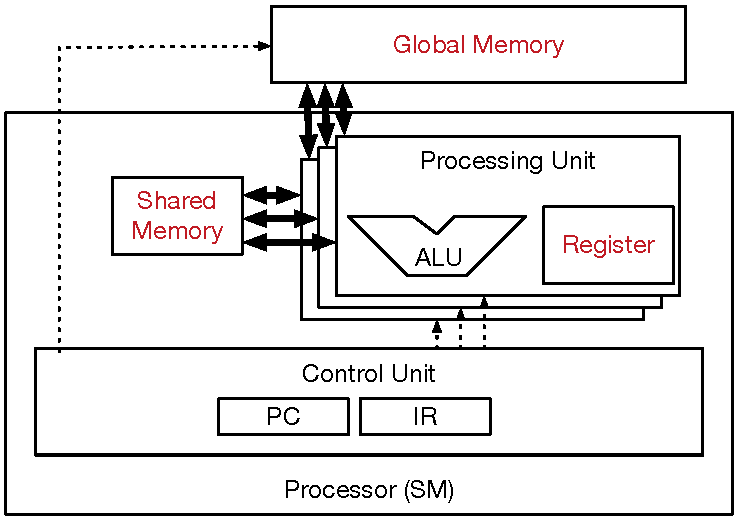
\includegraphics[scale=0.6]{./figures-pdf/hard_mem}
%\end{center}
%\end{frame}
%%%%%%%%%%%%%%%%%%%%%%%%%%
\begin{frame}[plain,fragile]
\frametitle{Mémoire CUDA vue par le programmeur}
\begin{center}
	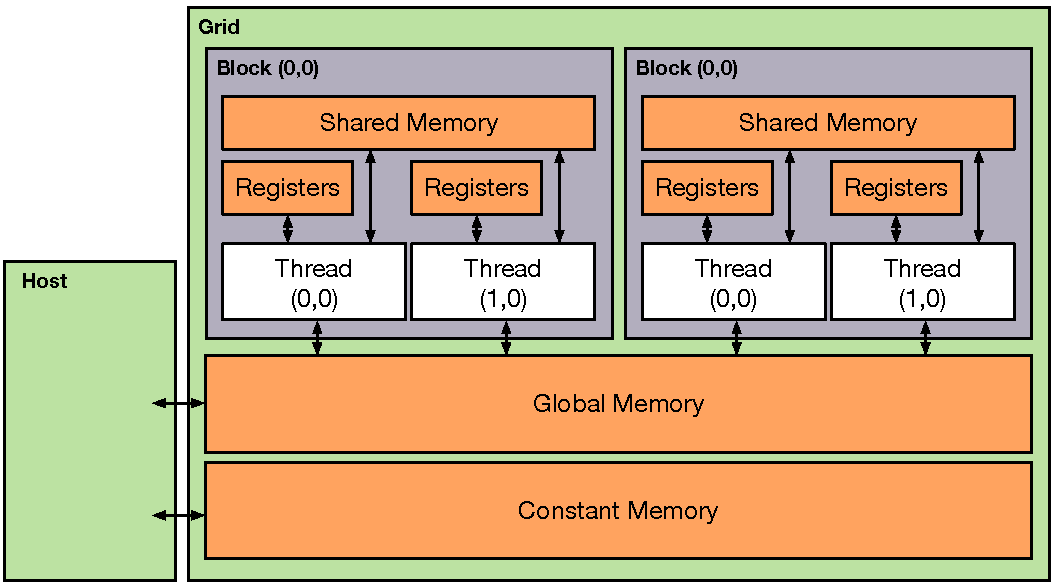
\includegraphics[scale=0.6]{./figures-pdf/prog_mem}
\end{center}
\end{frame}
%%%%%%%%%%%%%%%%%%%%%%%%%%
\begin{frame}[plain,fragile]
\frametitle{Focus {\it shared memory}}
La {\it shared memory} est une mémoire dont le contenu est explicitement déclaré et utilisé dans le code source d'un {\it kernel}.\medskip

Elle a les caractéristiques suivantes :
\begin{itemize}
	\item {\bf Accès à une vitesse beaucoup plus élevée (en termes de latence et de débit) que la mémoire globale}
	\item Présente dans chaque Streaming Multiprocessor (SM), i.e.unité de calcul
	\item Portée limitée aux threads qui compose un block
	\item Durée de vie du block, i.e. le contenu disparait une fois que les threads terminent leur exécution
%	\item Accès par instructions de chargement (load) et de stockage (store)
	\item Une forme de mémoire de type "scratchpad"
	\item Taille restreinte --- Jetson Nano : "Maximum amount of shared memory per SM 64 KB" et "Maximum amount of shared memory per thread block 48 KB"
\end{itemize}
\end{frame}
%%%%%%%%%%%%%%%%%%%%%%%%%%
\begin{frame}[plain,fragile]
\frametitle{Déclaration des variables en CUDA pour un kernel}
{\scriptsize \begin{table}[htdp]

\begin{center}
\begin{tabular}{|ll|c|c|c|}
\hline
 &&  Mémoire & Portée & Durée de vie\\
\hline
&{\tt int LocalVar;} & registre & thread & thread\\
{\tt \_\_device\_\_ \_\_shared\_\_}& {\tt int SharedVar;} & shared & block & block\\
{\tt \_\_device\_\_} & {\tt int GlobalVar;} & global & grid & application\\
{\tt \_\_device\_\_ \_\_constant\_\_} & {\tt int ConstantVar;} & constant & grid & application\\
\hline
\end{tabular}
\end{center}
\end{table}%
}
\begin{itemize}
	\item {\tt \_\_device\_\_} est optionnel avec {\tt \_\_shared\_\_} et {\tt \_\_constant\_\_}
\end{itemize}

Exemple
\begin{lstlisting}[language=C]
	__shared__ int vector[NB_ELT];
	__shared__ float ds_in[tileSize][tileSize];
 \end{lstlisting}
\end{frame}

%%%%%%%%%%%%%%%%%%%%%%%%%%
\begin{frame}[plain,fragile]
\frametitle{Exemple d'utilisation : produit matriciel}
\begin{center}
	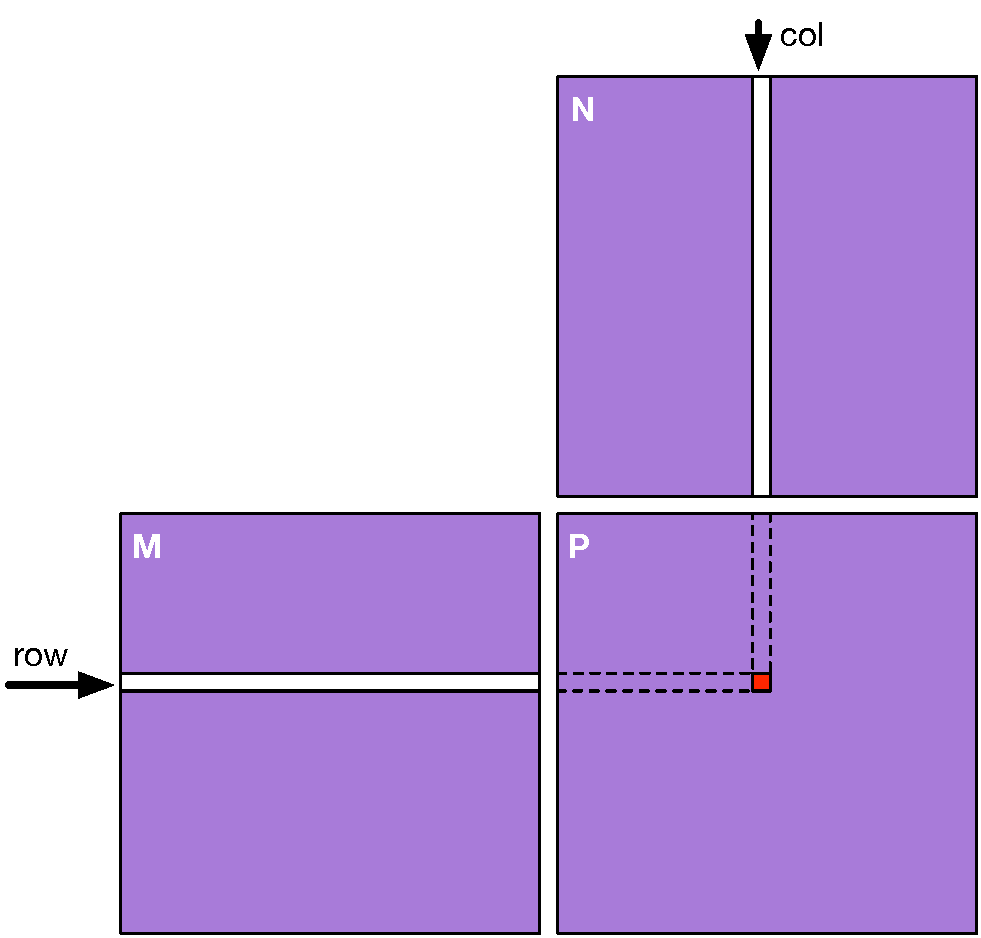
\includegraphics[scale=0.5]{./figures-pdf/mat_mul}
\end{center}
\end{frame}

%%%%%%%%%%%%%%%%%%%%%%%%%%
\begin{frame}[plain,fragile]
\frametitle{Kernel pour la multiplication matricielle : version naïve }
\begin{lstlisting}[language=C]

/**
 Naive Kernel for matrix product P = M*N
 To simplify writing, matrices are assumed to be square (size given by width)
*/

__global__
void MatrixMulKernel(float* M, float* N, float* P, int width)
{
  // Calculate the row index of the P element and M
  int row = blockIdx.y*blockDim.y+threadIdx.y;

  // Calculate the column index of P and N
  int col = blockIdx.x*blockDim.x+threadIdx.x;

  if ((row < width) && (col < width)) {
    float sum = 0;
    // each thread computes one element of the block sub-matrix
    for (int k = 0; k < width; k++)
    {
      sum += M[row * width + k]*N[k * width + col];
    }
    P[row*width+col] = sum;
  }
  
}
 \end{lstlisting}
 
 \begin{itemize}
	\item  Chaque Thread {\tt (row,col)} calcule $P_{row,col} = \sum_{k = 0..width-1} M_{row,k}N_{k,col}$
  \end{itemize}
\end{frame}
%%%%%%%%%%%%%%%%%%%%%%%%%%
\begin{frame}[plain,fragile]
\frametitle{Accès mémoire}
\begin{center}
	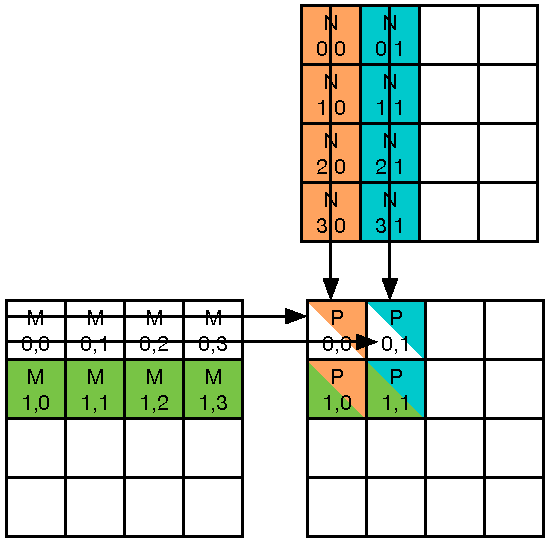
\includegraphics[scale=0.5]{./figures-pdf/calculation}
\end{center}
\begin{table}[htdp]
\begin{center}
\begin{tabular}{|c|c|c|c|c|}
\hline
thread$_{0,0}$ & {\color{red} $M_{0,0}$}$*N_{0,0}$ & {\color{red} $M_{0,1}$}$*N_{1,0}$ & {\color{red} $M_{0,2}$}$*N_{2,0}$ & {\color{red} $M_{0,3}$}$*N_{3,0}$  \\
\hline
thread$_{0,1}$ & {\color{red} $M_{0,0}$}$*N_{0,1}$ & {\color{red} $M_{0,1}$}$*N_{1,1}$ & {\color{red} $M_{0,2}$}$*N_{2,1}$ & {\color{red} $M_{0,3}$}$*N_{3,1}$  \\
\hline
\multicolumn{5}{c}{...}\\
\hline
thread$_{0,j}$ & {\color{red} $M_{0,0}$}$*N_{0,j}$ & {\color{red} $M_{0,1}$}$*N_{1,j}$ & {\color{red} $M_{0,2}$}$*N_{2,j}$ & {\color{red} $M_{0,3}$}$*N_{3,j}$  \\
\hline
\end{tabular}
\end{center}
\label{default}
\end{table}%
\end{frame}
%%%%%%%%%%%%%%%%%%%%%%%%%%
\begin{frame}[plain,fragile]
\frametitle{Accès mémoire}
\begin{center}
	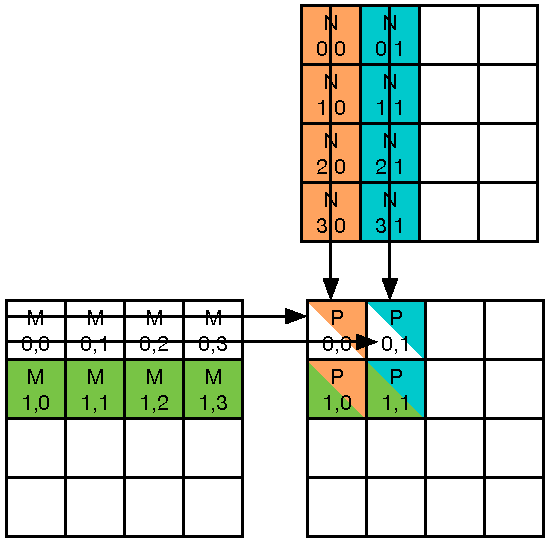
\includegraphics[scale=0.5]{./figures-pdf/calculation}
\end{center}
\begin{table}[htdp]
\begin{center}
\begin{tabular}{|c|c|c|c|c|}
\hline
thread$_{0,0}$ & {$M_{0,0}$}$*{\color{red} N_{0,0}}$ & {$M_{0,1}$}$*{\color{red} N_{1,0}}$ & { $M_{0,2}$}$*{\color{red} N_{2,0}}$ & {$M_{0,3}$}$*{\color{red}N_{3,0}}$  \\
\hline
thread$_{1,0}$ & {$M_{1,0}$}$*{\color{red} N_{0,0}}$ & {$M_{2,1}$}$*{\color{red} N_{1,0}}$ & { $M_{3,2}$}$*{\color{red} N_{2,0}}$ & {$M_{4,3}$}$*{\color{red}N_{3,0}}$  \\
\hline
\multicolumn{5}{c}{...}\\
\hline
thread$_{i,0}$ & {$M_{i,0}$}$*{\color{red} N_{0,0}}$ & {$M_{i,1}$}$*{\color{red} N_{1,0}}$ & { $M_{i,2}$}$*{\color{red} N_{2,0}}$ & {$M_{i,3}$}$*{\color{red}N_{3,0}}$  \\
\hline
\end{tabular}
\end{center}
\label{default}
\end{table}%
\end{frame}
%%%%%%%%%%%%%%%%%%%%%%%%%%
\begin{frame}[plain,fragile]
\frametitle{Utilisation de la mémoire partagée : produit matriciel}

\begin{itemize}
	\item<1-> {\bf Principe :} Pré-charger les données dans la mémoire partagée (1 seul accès mémoire par donnée) puis on réalise les calculs\bigskip
	
	\item<2-> {\bf Problème :} la mémoire partagée est limitée (64 ko au total ou 48ko/block), si les matrices sont grandes il n'est pas possible de tout pré-charger. Pour une donnée de 4 octets, vous pouvez seulement avoir 12000 valeurs par block. Dans notre cas cela correspond à deux matrices de 77x77. S'il y a quatre blocks, la limite est de 16ko par block, soit des matrices de 63x63.\bigskip
	\item<2-> {\bf Solution :} découpage en tuiles
\end{itemize}


\end{frame}
%%%%%%%%%%%%%%%%%%%%%%%%%%
\begin{frame}[plain,fragile]
\frametitle{Principe de la multiplication matricielle par tuile}

On utilise le fait que (sans les tests au bord) :\medskip
\begin{align*}
P_{row,col} 	&= 	\sum_{k = 0}^{width-1} M[row,k] \times N[k,col]\\
			&= 	\sum_{p = 0}^{\frac{width-1}{tileSize}} \sum_{k = 0}^{tileSize} M[row, p*tileSize+k] \times N[p*tileSize+k,col]
\end{align*}

\end{frame}
%%%%%%%%%%%%%%%%%%%%%%%%%%
\begin{frame}[plain,fragile]
\frametitle{Multiplication matricielle par tuile\\Tiled multiplication matrix}

\begin{itemize}
	\item Chaque thread réalise le calcul d'un élément de la matrice produit $P$
	\item Les threads sont regroupés par block de taille {\tt tileSize $\times$ tileSize}
	\item Le calcul est divisé en {\tt p} étapes qui réalisent :
	\begin{itemize}
		\item Le chargement  en mémoire partagée  d'une tuile de M et d'une de N de taille {\tt tileSize $\times$ tileSize}
		\item La somme des produits de ces sous-matrices
	\end{itemize}
\end{itemize}

\begin{center}
	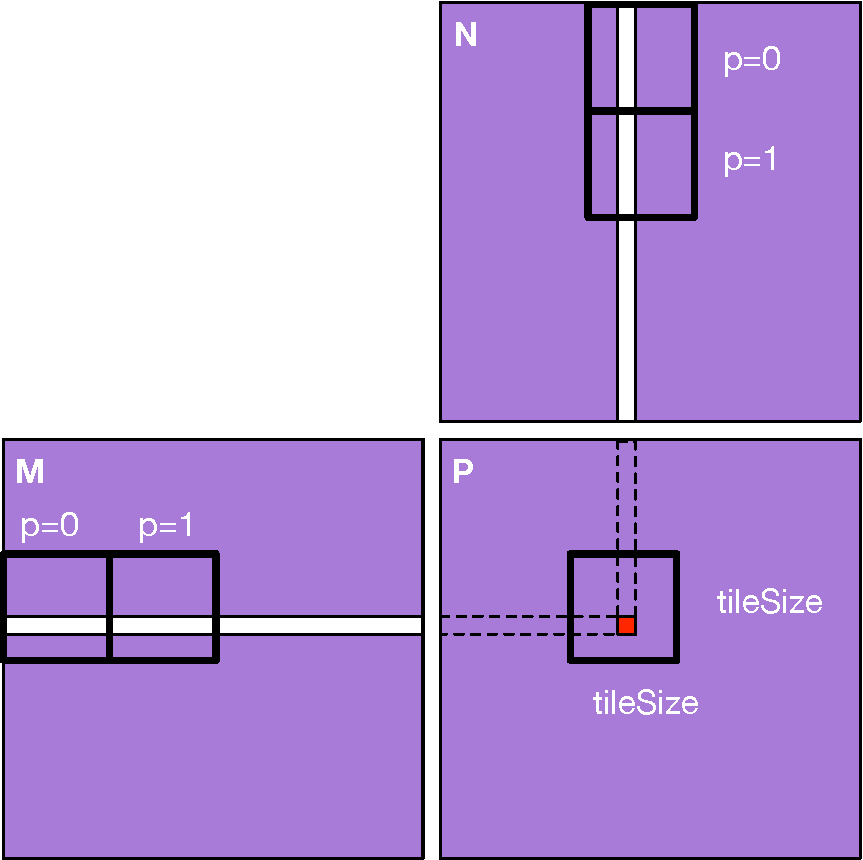
\includegraphics[scale=0.3]{./figures-pdf/tiled}
\end{center}
\end{frame}
%%%%%%%%%%%%%%%%%%%%%%%%%%
\begin{frame}[plain,fragile]
\frametitle{Multiplication matricielle par tuile (phase p=0)}
\begin{center}
	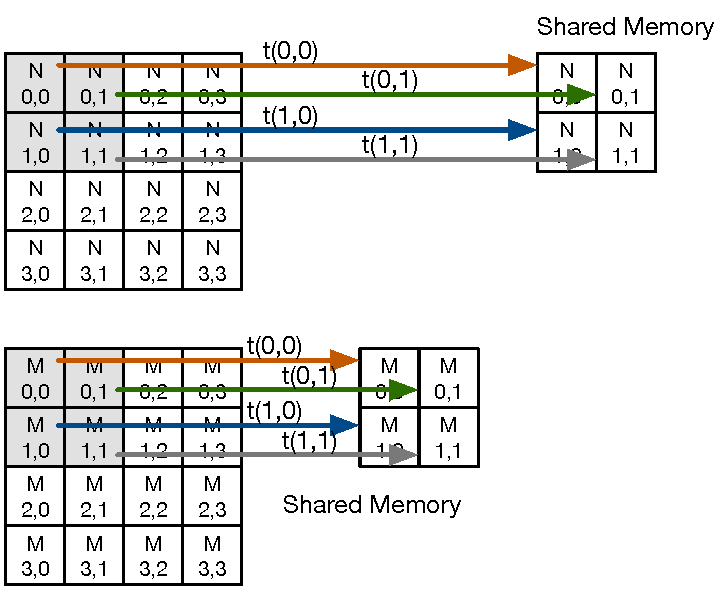
\includegraphics[scale=0.5]{./figures-pdf/phase0_load}
\end{center}
\end{frame}
%%%%%%%%%%%%%%%%%%%%%%%%%%
\begin{frame}[plain,fragile]
\frametitle{Multiplication matricielle par tuile (phase 0)}
\begin{center}
	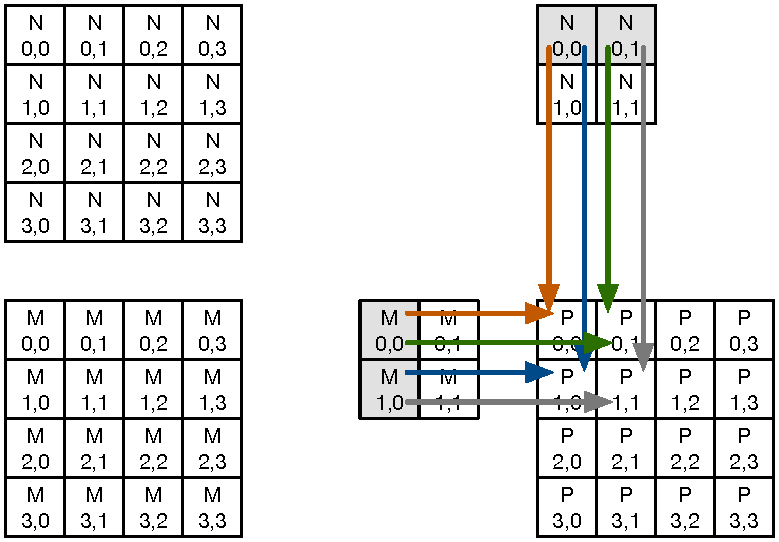
\includegraphics[scale=0.5]{./figures-pdf/phase0_use0}
\end{center}
\end{frame}
%%%%%%%%%%%%%%%%%%%%%%%%%%
\begin{frame}[plain,fragile]
\frametitle{Multiplication matricielle par tuile (phase p=0)}
\begin{center}
	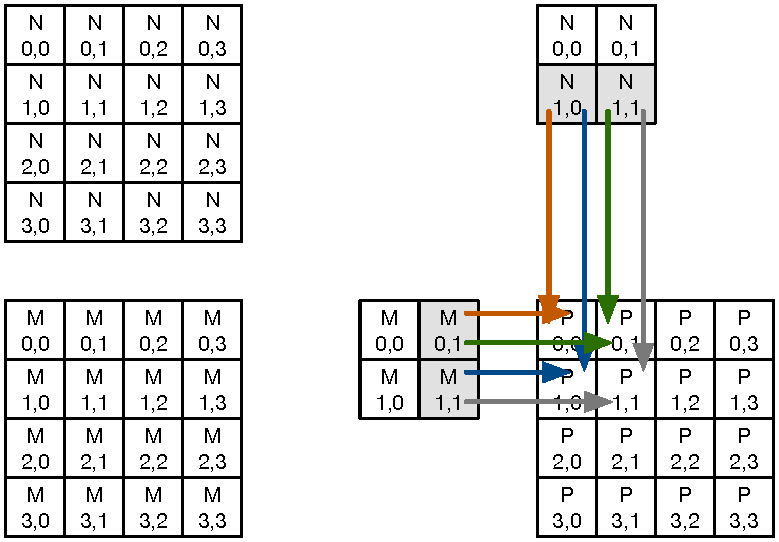
\includegraphics[scale=0.5]{./figures-pdf/phase0_use1}
\end{center}
\end{frame}
%%%%%%%%%%%%%%%%%%%%%%%%%%
\begin{frame}[plain,fragile]
\frametitle{Multiplication matricielle par tuile (phase p=1)}
\begin{center}
	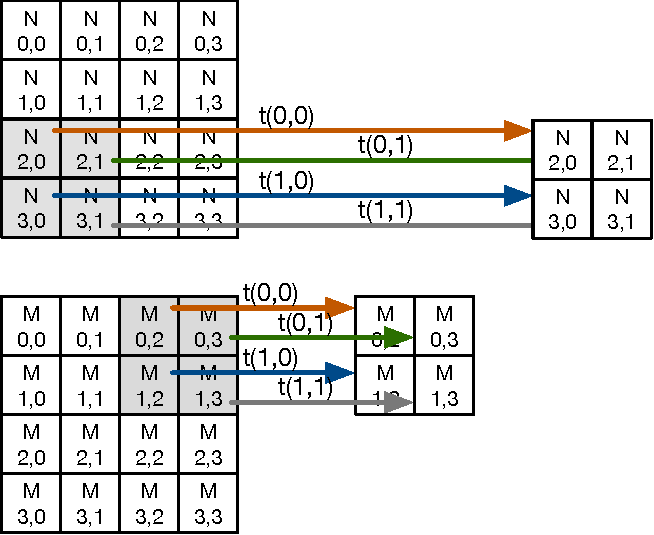
\includegraphics[scale=0.5]{./figures-pdf/phase1_load}
\end{center}
\end{frame}
%%%%%%%%%%%%%%%%%%%%%%%%%%
\begin{frame}[plain,fragile]
\frametitle{Code du kernel}
\begin{lstlisting}[language=C]

#define tileSize 32

__global__
void MatrixMulKernel(float* M, float* N, float* P, int width)
{
  // Defining shared memory workspaces
  __shared__ float ds_M[tileSize][tileSize];
  __shared__ float ds_N[tileSize][tileSize];
  
  // Redefinition of blockIdx.x, blockIdx.y, 
  // threadIdx.x and threadIdx.y to simplify writing
  int bx = blockIdx.x; int by  = blockIdx.y;
  int tx = threadIdx.x; int ty = threadIdx.y;
  
  // Definition of row and col
  int row = by * blockDim.y + ty;
  int col = bx * blockDim.x + tx;

  // intermediate variable for calculating the sum of products  
  float sum = 0.0;
  
  // Loop over the M and N tiles required to compute the P element
  for (int p = 0; p < width / tileSize; p++) {
    // collaborative loading of M and N tiles into shared memory
    ds_M[ty][tx] = M[row * width + p * tileSize + tx];
    ds_N[ty][tx] = N[(p * tileSize + ty) * width + col];
  
    for (int k = 0; k < tileSize; k++)
    {
    	sum+= ds_M[ty][k] * ds_N[k][tx];
    }
  }
  P[row * width + col] = sum;
}

 \end{lstlisting}

\end{frame}
%%%%%%%%%%%%%%%%%%%%%%%%%%
\begin{frame}[plain,fragile]
\frametitle{Attention dangers : synchronisation}
      \begin{block}{}
	Que se passe-t-il si un thread (d'un autre warp) n'a pas chargé la mémoire avant de commencer les calculs ?
\end{block}  

\begin{center}
	{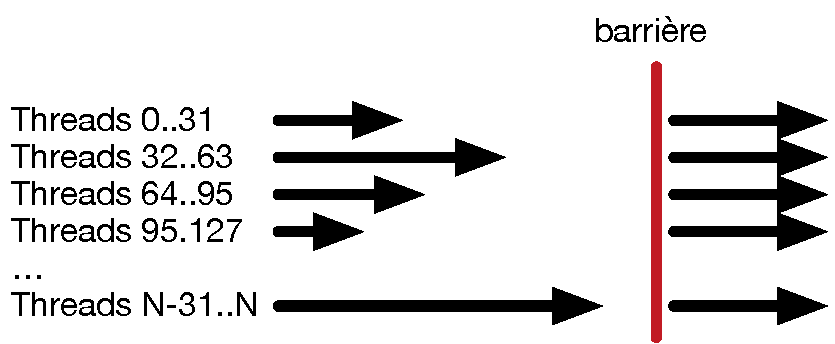
\includegraphics[scale=0.5]{./figures-pdf/barriere}}
\end{center}

      \begin{block}{}

\begin{lstlisting}[language=C]
  // synchronize threads in this block
  __syncthreads();
 \end{lstlisting}
Garantit que chaque {\bf thread du { block}} a terminé ses instructions après l'appel à {\tt \_\_syncthreads()}
\end{block}
\end{frame}
%%%%%%%%%%%%%%%%%%%%%%%%%%
%\begin{frame}[plain,fragile]
%\frametitle{Le problème de congestion}
%      \begin{block}{}
%	Pour résoudre le problème des embouteillages :
%	\begin{itemize}
%		\item<2-> co-voiturage (regroupement des demandes)
%		\item<3> emploi du temps (synchronisation de l'utilisation des données)
%	\end{itemize}
%\end{block}  
%\end{frame}
%%%%%%%%%%%%%%%%%%%%%%%%%%
\begin{frame}[plain,fragile]
\frametitle{Exemple avec la multiplication matricielle (carré) : kernel}
\begin{lstlisting}[language=C]

__global__
void MatrixMulKernel(float* M, float* N, float* P, int width)
{
  __shared__ float ds_M[tileSize][tileSize];
  __shared__ float ds_N[tileSize][tileSize];
  
  int bx = blockIdx.x; int by  = blockIdx.y;
  int tx = threadIdx.x; int ty = threadIdx.y;
  
  int row = by * blockDim.y + ty;
  int col = bx * blockDim.x + tx;
  float sum = 0.0;
  
  for (int p = 0; p < width / tileSize; p++) {
    ds_M[ty][tx] = M[row * width + p * tileSize + tx];
    ds_N[ty][tx] = N[(p * tileSize + ty) * width + col];
    
     // Synchronization to ensure that shared memory has been 
     // fully loaded by all threads before starting calculations
    __syncthreads();
  
    for (int i = 0; i < tileSize; ++i)
    {
    	sum+= ds_M[ty][i] * ds_N[i][tx];
    }
    
   // Synchronization to ensure that shared memory is not 
   // modified before calculations are completed for all threads
    __syncthreads();
  }
  P[row * width + col] = sum;
}
 \end{lstlisting}

\end{frame}
%%%%%%%%%%%%%%%%%%%%%%%%%%
\begin{frame}[plain,fragile]
\frametitle{Considérations sur la taille des tuiles (block de threads)}

\begin{itemize}
	\item Supposons deux valeurs pour  {\tt tileSize} :
	\begin{itemize}
		\item 16 : ce qui donne $16 \times 16 = 256$ threads par block
		\item 32 : ce qui donne $32 \times 32 = 1024$ threads par block
	\end{itemize}
	\item Pour 16, à chaque phase, chaque block effectue $2 \times 256 = 512$ chargements de flottants depuis la mémoire globale pour $256 \times (2 \times 16) = 8 192$ opérations mul/add, soit 16 opérations à virgule flottante pour chaque chargement de mémoire
	\item Pour 32, dans chaque phase, chaque block effectue $2 \times 1024 = 2048$ chargements de flottants depuis la mémoire globale pour $1024 \times (2 \times 32) = 65 536$ opérations mul/add, soit {\bf 32 opérations à virgule flottante pour chaque chargement de mémoire}

\end{itemize}
\end{frame}
%%%%%%%%%%%%%%%%%%%%%%%%%%
\begin{frame}[plain,fragile]
\frametitle{Shared Memory et Threading}

Lien : \href{https://docs.nvidia.com/cuda/cuda-c-programming-guide/index.html#compute-capabilities}{compute capabilities} (SM avec 64 Ko de mémoire partagée)

\begin{itemize}
	\item La taille de la mémoire partagée dépend de l'implémentation !
	\item Pour {\tt tileSize}=16, chaque block de threads utilise 2*256*4o=2Ko de mémoire partagée
		\begin{itemize}
		\item Pour une mémoire partagée de 64 Ko, on peut potentiellement avoir jusqu'à 32 blocks de threads qui exécutent des opérations
		\item Cela permet jusqu'à 32*512 = 16 384 chargements mémoire simultanés (2 par thread, 256 threads par block)
	\end{itemize}
	\item Pour tileSize=32, chaque block de thread utilise 2*32*32*4o=8Ko de mémoire partagée
	\begin{itemize}
		\item Pour une mémoire partagée de 64 Ko, on peut potentiellement avoir jusqu'à 8 blocks de threads qui exécutent des opérations
		\item Cela permet jusqu'à 8*2048 = 65 536 chargements mémoire simultanés (2 par thread, 1024 threads par block)
	\end{itemize}
	\item Chaque \_\_syncthread() peut réduire le nombre de warps actifs pour un block : un grand nombre de blocks peut être avantageux



\end{itemize}
\end{frame}

%%%%%%%%%%%%%%%%%%%%%%%%%%
\begin{frame}[plain,fragile]
\frametitle{Généralisation : technique de décomposition en tuiles}

Si plusieurs threads font fréquemment des accès à des données communes, on découpe l'algorithme de traitement en plusieurs phases. A chaque phase :
\begin{enumerate}
	\item on charge les données de la mémoire globale dans une mémoire partagée, puis 
	\item on réalise les calculs sur ce sous-ensemble de valeurs.
\end{enumerate}
\medskip

L'objectif est de réduire l'effet limitatif de la bande passante mémoire sur les performances des kernels.

\begin{center}
	\only<1>{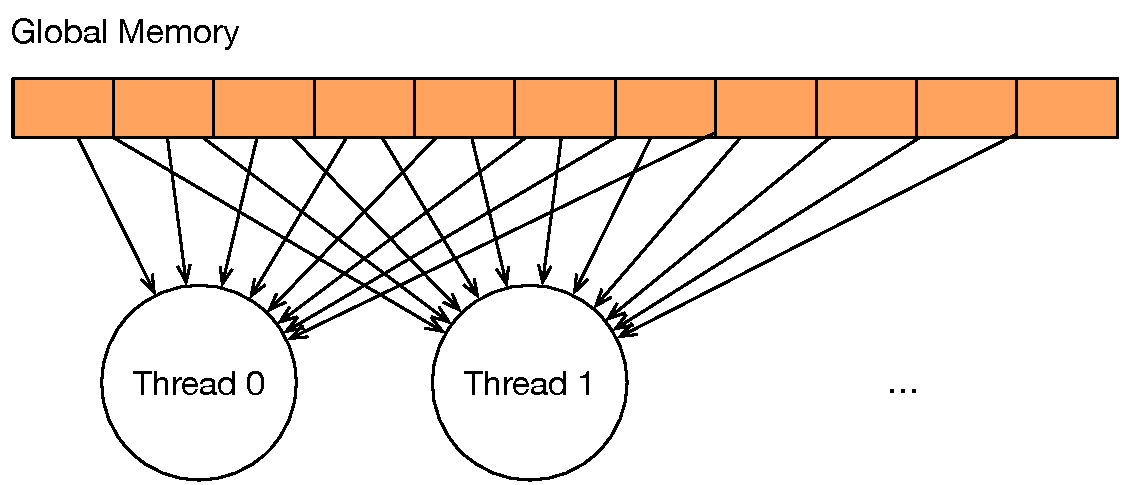
\includegraphics[scale=0.5]{./figures-pdf/global}}
	\only<2>{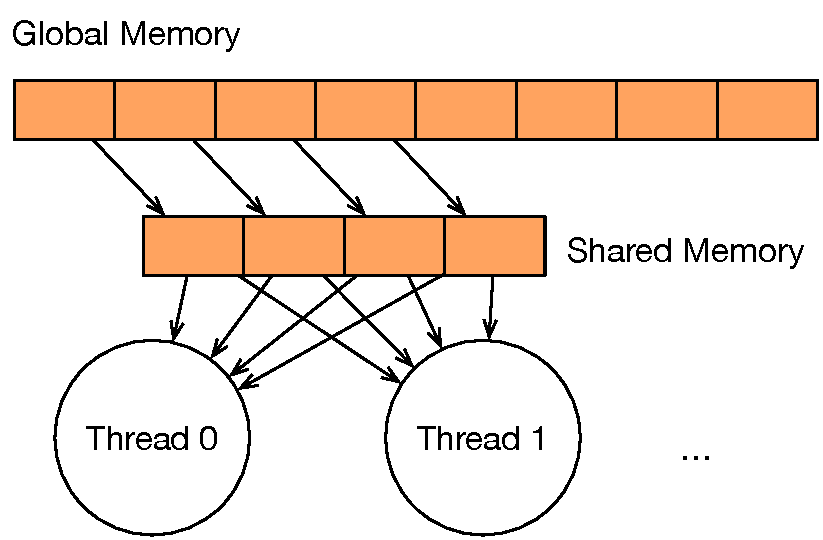
\includegraphics[scale=0.5]{./figures-pdf/tiled1}}
	\only<3>{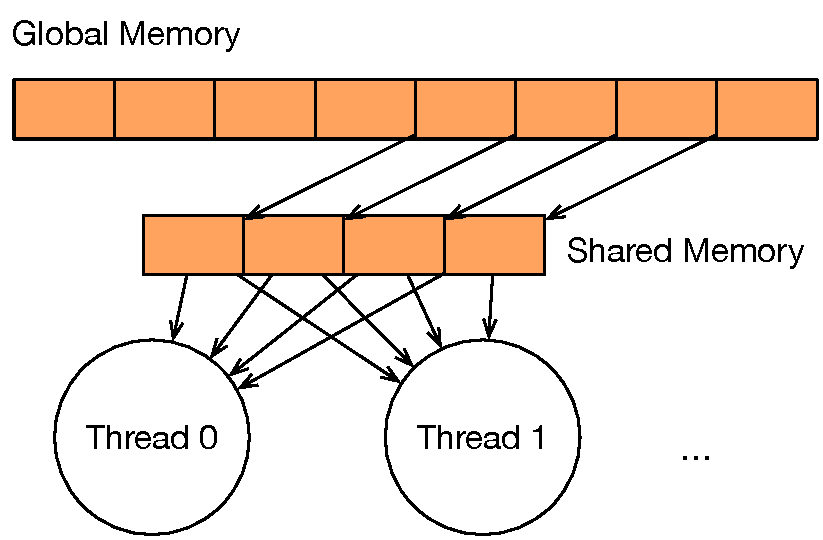
\includegraphics[scale=0.5]{./figures-pdf/tiled2}}
\end{center}
\end{frame}
%%%%%%%%%%%%%%%%%%%%%%%%%%
%\begin{frame}[plain,fragile]
%\frametitle{Le calcul avec des tuiles dans les grandes lignes}
%\begin{itemize}
%\item Identifier une tuile de la mémoire globale qui est utilisée par de multiples threads
%\item Charger la tuile de la mémoire globale dans la mémoire sur le SM
%\item Utiliser la synchronisation des barrières pour s'assurer que tous les threads ont finis le chargement mémoire
%\item Avoir plusieurs threads pour accéder à leurs données à partir de la mémoire partagée
%\item Utiliser la synchronisation des barrières pour s'assurer que tous les threads ont terminé leur calcul
%\item Passer à la tuile suivante
%\end{itemize}
%
%\end{frame}

%%%%%%%%%%%%%%%%%%%%%%%%%%
\begin{frame}[plain,fragile]
\frametitle{Retour sur la multiplication de matrices : gérer la taille des matrices}

\begin{block}{}
 \begin{itemize}
 	\item {\bf Problème :} Que faire pour les valeurs dans une tuile qui est en dehors de la matrice ?
 	\item {\bf Solution :} on charge une valeur de 0.0 en mémoire partagée
 \end{itemize}
\end{block}


\begin{lstlisting}[language=C]

__global__
void MatrixMulKernel(float* M, float* N, float* P, int width) // square matrix
{
  ...
  for (int p = 0; p < (width-1)/tileSize + 1; ++p) {
    if(row < width && ty * tileSize+tx < width)
	{ ds_M[ty][tx] = M[row*width + p*tileSize+tx]; }
    else 
    	{ ds_M[ty][tx] = 0.0; } // Load default value 0.0
    if (p*tileSize+ty < width && col < width) 
	{ ds_N[ty][tx] = N[(t*tileSize+ty)*width + col]; }
    else
    	{ ds_M[ty][tx] = 0.0; } // Load default value 0.0
    __syncthreads();
    
    if(row < width && col < width) {
	for (int i = 0; i < tileSize; ++i)
		{ sum+= ds_M[ty][i] * ds_N[i][tx]; }
    }
    __syncthreads();
  }
  if (row < width && col < width)
	  { P[row*width+col] = sum; }
}
 \end{lstlisting}
 
% \begin{block}{}
%Cette approche ce généralise à des dimension quelconque de matrice.
%\end{block}


\end{frame}

%%%%%%%%%%%%%%%%%%%%%%%%%%
\begin{frame}[plain]
\frametitle{Un peu de pratique avec le TD 5}

\begin{block}{Objectifs}
\begin{itemize}
	\item Utiliser des mécanismes de synchronisation
	\item Utiliser la mémoire partagée
	\item Mettre en place une décomposition en tuile
\end{itemize}
\end{block}
\end{frame}
%%%%%%%%%%%%%%%%%%%%%%%%%%

%%%%%%%%%%%%%%%%%%%%%%%%%%
\end{document}